\documentclass[a4paper,14pt]{extarticle} 
\usepackage[a4paper,top=1.5cm, bottom=1.5cm, left=2cm, right=1cm]{geometry}
%\usepackage[T2A]{fontenc}
%\usepackage[english, russian]{babel}
\usepackage{graphicx}
\graphicspath{{./pics/}}
\DeclareGraphicsExtensions{.pdf,.png,}
\usepackage[table]{xcolor}

\usepackage{fontspec}
\setmainfont{Times New Roman}
\setsansfont{FreeSans}
\setmonofont{FreeMono}
\renewcommand{\baselinestretch}{1.5}
\usepackage{polyglossia}
\setdefaultlanguage{russian}
\setotherlanguages{english,russian}
\usepackage{setspace}
\usepackage[many]{tcolorbox}
\usepackage{array}
\usepackage{longtable}
\usepackage{multicol} 
\usepackage{caption}

\begin{document}
    \begin{center}
        \thispagestyle{empty}
        \begin{singlespace}
        ФЕДЕРАЛЬНОЕ АГЕНТСТВО СВЯЗИ

        ФЕДЕРАЛЬНОЕ ГОСУДАРСТВЕННОЕ БЮДЖЕТНОЕ ОБРАЗОВАТЕЛЬНОЕ

        УЧРЕЖДЕНИЕ ВЫСШЕГО ОБРАЗОВАНИЯ

        «САНКТ-ПЕТЕРБУРГСКИЙ ГОСУДАРСТВЕННЫЙ УНИВЕРСИТЕТ ТЕЛЕКОММУНИКАЦИЙ ИМ. ПРОФ. М.А. БОНЧ-БРУЕВИЧА»

        (СПбГУТ)
        \end{singlespace}
        \vspace{-1ex}
        \rule{\textwidth}{0.4pt}
        \vspace{-5ex}

        \vspace{100px}
        \textbf{Лабораторная работа №5}\\
        ИССЛЕДОВАНИЕ СХЕМ НА ИНТЕГРАЛЬНОМ ОУ В ЧАСТОТНОЙ И ВРЕМЕННОЙ ОБЛАСТЯХ
        \begin{center}
            Вариант 234
        \end{center}
    \vspace{100px}
    \end{center}
    \vspace{4ex}
    \begin{flushright}
    \parbox{12 cm}{
    \begin{flushleft}
        Выполнила бригада:\\
        Группа ИКТЗ-83\\
        \underline{Громов А.А., Миколаени М.С., Мазеин Д.С.} \hfill \rule[-0.85ex]{0.09\textwidth}{0.6pt}\\
        \vspace{-1ex}
        \footnotesize \textit{ (Ф.И.О., № группы) \hfill (подпись)} \normalsize


    \end{flushleft}
    }
    \end{flushright}
    \begin{center}
        \vfill
        Санкт-Петербург

        2020

    \end{center}
    \newpage


    \begin{center}
        \begin{singlespace}
             Лабораторная работа № 5

            \textbf{“Исследование схем на интегральном ОУ в частотной и временной областях”}           
        \end{singlespace}
    \end{center}
    \textbf{\underline{Цель работы}}: 
    \vspace{-1cm}
    \begin{singlespace}
        \begin{itemize}
            \item Изучить схемотехнические особенности построения интегральных ОУ, принцип построения макромодели в частотной области.
            \item Исследовать влияние внешних цепей ОС на характеристики устройств с ОУ.
        \end{itemize}
    \end{singlespace}
    
    \textbf{Иходные данные:}\\
    Таблица 4\\
    \begin{tabular}{|c|c|>{\centering}m{3.5cm}|>{\centering}m{3.5cm}|>{\centering}m{3.5cm}|>{\centering}m{3.5cm}|}
    \hline
    № & Тип ОУ & Частота единичного усиления (МГц) & Коэффициент усиления ОУ (дБ) & Скорость нарастания (В/мкс) & Максимальный выходной ток (мА)
    \tabularnewline
    \hline
    2 & ОРА646 & 650 & 47 & 180 & 52
    \tabularnewline
    \hline
    \end{tabular}\\

    Таблица 5\\
    \begin{tabular}{|c|c|}
    \hline
    № & 3
    \tabularnewline
    \hline
    R, кОм & 1.6
    \tabularnewline
    \hline
    C, пФ & 100
    \tabularnewline
    \hline
    \end{tabular}\\

    Таблица 6\\
    \begin{tabular}{|c|c|}
    \hline
    № & 4
    \tabularnewline
    \hline
    R, кОм & 4.7
    \tabularnewline
    \hline
    C, нФ & 68
    \tabularnewline
    \hline
    \end{tabular}\\

    \newpage
    \begin{center}
        \textbf{2.1. Построение макромодели ОУ с частотной коррекцией.}
    \end{center}
    
    Модель, удобная для учебного процесса, показана на рис. 1. Элементы 
    частотной коррекции не показаны. Схема, однако, обладает свойствами 
    скорректированного ОУ, в частности ее характеристики определяются 
    двумя полюсами в функции передачи.

    Эта модель состоит из трех блоков, построенных на идеальных 
    операционных усилителях. Первый (ОУ1) обеспечивает дифференциальный 
    вход устройства с бесконечно большим входным сопротивлением. Третий 
    (ОУ3) обеспечивает нулевое выходное сопротивление и служит буфером 
    между выходом макромодели и внешними цепями. Частотные свойства в 
    предложенной макромодели ОУ определяются двумя парами ВС-элементов на 
    выходах ОУ1 и ОУ2 (узлы 4 и 5). Общий коэффициент усиления макромодели 
    ОУ указывается над ОУ1. Другие блоки имеют коэффициент усиления равный 1.

    \newpage

    \begin{center}
        \textbf{Задание 1.}
    \end{center}

    Составим макромодель по заданным параметрам:

    Коэффициент усиления ОУ μ указывается над ОУ1, другие блоки имеют 
    усиление 1. Ёмкости, связанные с частотами полюсов, определяются из 
    выражения $C_i=1/2πf_{pi}R$.\\
    \vspace{-1cm}
    \begin{multicols}{2}
    \noindent $f_1$ = 650 МГц\\
    KдБ = 47 дБ\\
    μ = 224\\
    \columnbreak
    $f_{p1}$ = 2.9 МГц\\
    $f_{p2}$ = $f_1$ ∙ 2 = 1.3ГГц\\
    $C_i$ = $\frac{1}{2}$ \cdot π\cdot $f_{pi}$ \cdot R\\
    $C_1$ = 55 нФ\\
    $C_2$ = 0.1224 пФ\\
    \end{multicols}
    \begin{figure}[h!]
        \begin{center}
            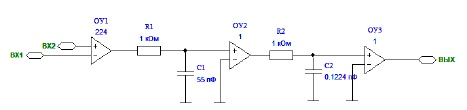
\includegraphics[scale=0.9]{1.png}
            \caption{Макромодель с параметрами элементов, задающих частотные свойства ОУ.}
        \end{center}
    \end{figure}

    \newpage
    \begin{center}
        \textbf{3.2.1. Схемы на ОУ с частотно-независимой ОС.}
    \end{center}

    \textbf{Неинвертирующий усилитель с ОС} изображен на рис. 2, а. В этой
    схеме сигнал подается на прямой вход ОУ. Напряжение отрицательной ОС поступает на инверсный вход ОУ. Цепь ОС из резисторов R1 и R2 образует
    последовательную ОС по входу и параллельную по выходу. Коэффициент
    усиления $К_{FH}$ этой структуры записан под схемой. Здесь и собственный
    коэффициент усиления ОУ без ОС, F - глубина ОС.

    \textbf{Инвертирующий усилитель с ОС} изображен на рис. 2, 6. В этой схе-
    ме сигнал через резистор R1 подается на инверсный вход ОУ. На этот же
    вход должен поступать и сигнал ОС, иначе она не будет отрицательной.
    Таким образом, и в инвертирующем включении ОУ цепь ОС образуется
    резисторами R1 и R2. При этом получается параллельная по инверсному
    входу ОУ и параллельная по выходу ОС. Коэффициент усиления КFH этой
    структуры также записан под соответствующей схемой. Глубина ОС в обеих
    схемах одинакова.
    \begin{center}
        $K_{FH}=\frac{\mu}{F}\approx 1+\frac{R2}{R1}$; $K_\text{Fи}=\frac{R2}{R1+R2}\frac{\mu}{F}\approx \frac{R2}{R1}$\\
        $F=1+\mu B=1+\mu \frac{R1}{R1+R2}$.   
    \end{center}
    \begin{figure}[h!]
        \begin{center}
            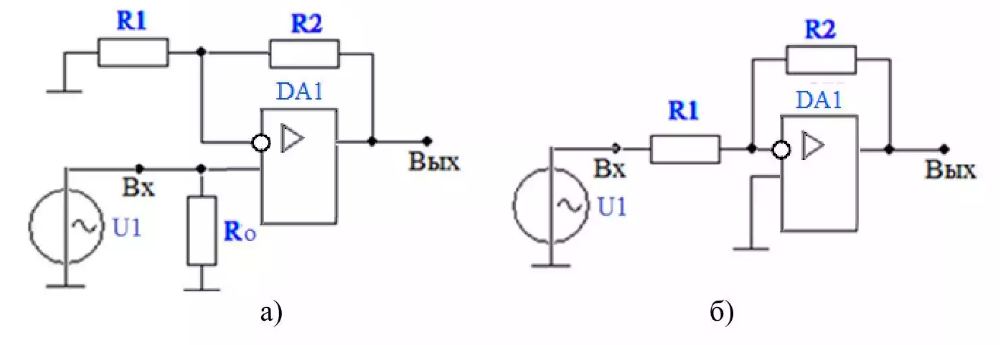
\includegraphics[scale=0.5]{3.png}
        \end{center} 
        \caption{Основные схемы включения операционных усилителей.}
    \end{figure}
    \newpage

    \begin{center}
        \textbf{3.2.1.1. Характеристики в частотой области.}
    \end{center}

    Режим без ОС можно создать, подключив к одному из входов подсхемы ОУ 
    (рис. 3) источник гармонического сигнала (с амплитудой 1...2 мВ) и 
    заземлив другой. В этом случае исследованию подвергается 
    собственно сама микросхема ОУ.

    \begin{figure}[h!]
        \begin{center}
            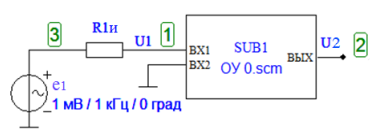
\includegraphics{4.png}
        \end{center}
        \caption{Схема включения ОУ без ОС.}
    \end{figure}
    
    \begin{center}
        \textbf{Задание 2.}
    \end{center}

    Построить АЧХ ОУ без ОС, определить коэффициент усиления μ на нижних 
    частотах (20…80 Гц), частоты полюсов и частоту единичного усиления f1.

    \begin{figure}[h!]
        \begin{center}
            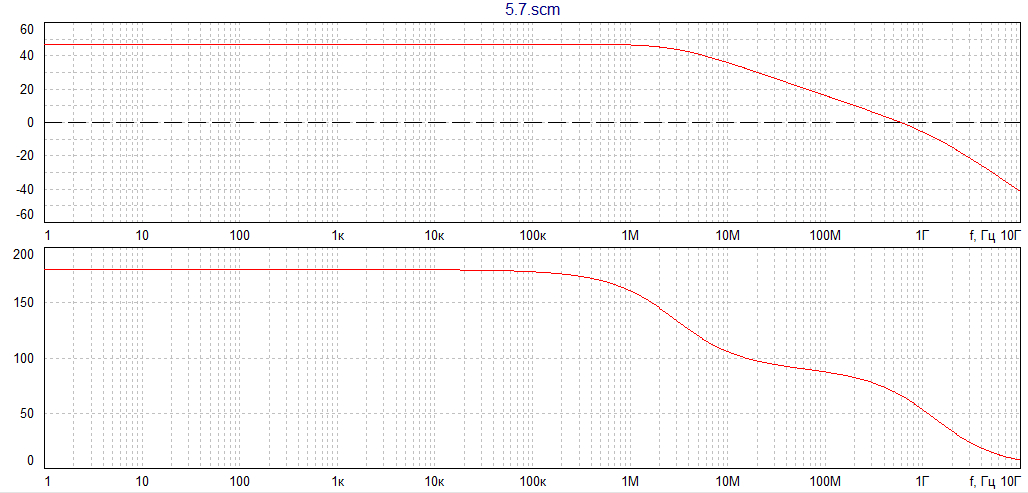
\includegraphics[scale=0.6]{5.png}
        \end{center}
        \caption{Частотные характеристики ОУ.}
    \end{figure}

    \begin{center}
        \mu = 224, $f_{P1}$=2.9 МГц, $f_{P2}$=1.3 ГГц, $f_1$=640 МГц
    \end{center}

    \vspace{-0,5cm}
    Режим ОУ с ОС получается при подключении к подсхеме резисторов ОС R1 и 
    R2 (рис. 5). Для получения заданных коэффициентов усиления с ОС $K_F$, 
    равными 100 и 10, необходимо включить требуемые сопротивления 
    резисторов ОС. Их можно рассчитать, приняв R1 = 1...2 кОм.

    Если источник сигнала подключается к инверсному входу ОУ через
    резистор R1. Получаем инвертирующий усилитель (рис. 5).

    \begin{figure}[h!]
        \begin{center}
            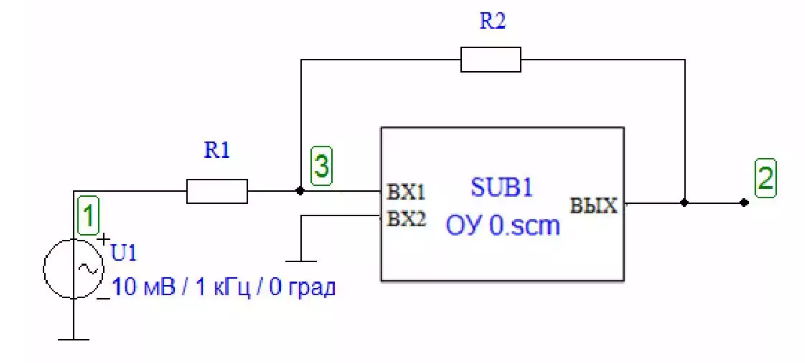
\includegraphics[scale=0.5]{6.png}
        \end{center}
        \vspace{-1cm}
        \caption{Инвертирующий усилитель.}
    \end{figure}

    \textbf{Вывод по заданию:}

    \begin{itemize}
        \item Рассчитанные и полученные по АЧХ частоты полюсов совпадают, а
              частота единичного усиления практически совпадает с 
              теоретической.
        \item Условия сдвига фаз по ФЧХ для каждого полюса совпадают с 
              теоретическими требованиями к фЧХ двуполюсного усилителя.
    \end{itemize}
    \newpage
    \begin{center}
        \textbf{Задание 3.}
    \end{center}

    \begin{figure}[h!]
        \captionsetup{justification=centering}
        \begin{center}
            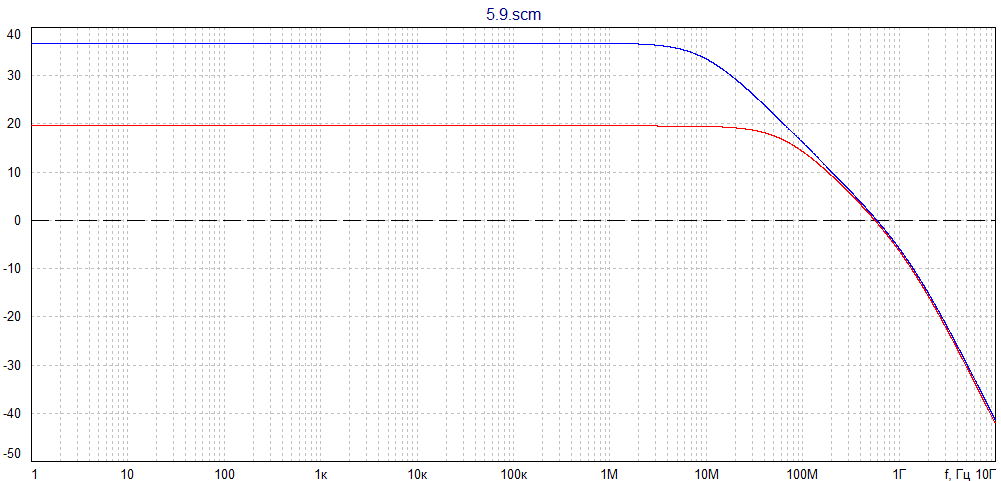
\includegraphics[scale=0.6]{7.png}
        \end{center}
        \caption{График АЧХ. Красная линия- $K_F$=10; $f_\text{гран}$=64МГц | Синяя линия- $K_F$=100; $f_\text{гран}$=9.3 МГц.}
    \end{figure}

    \begin{figure}[h!]
        \begin{center}
            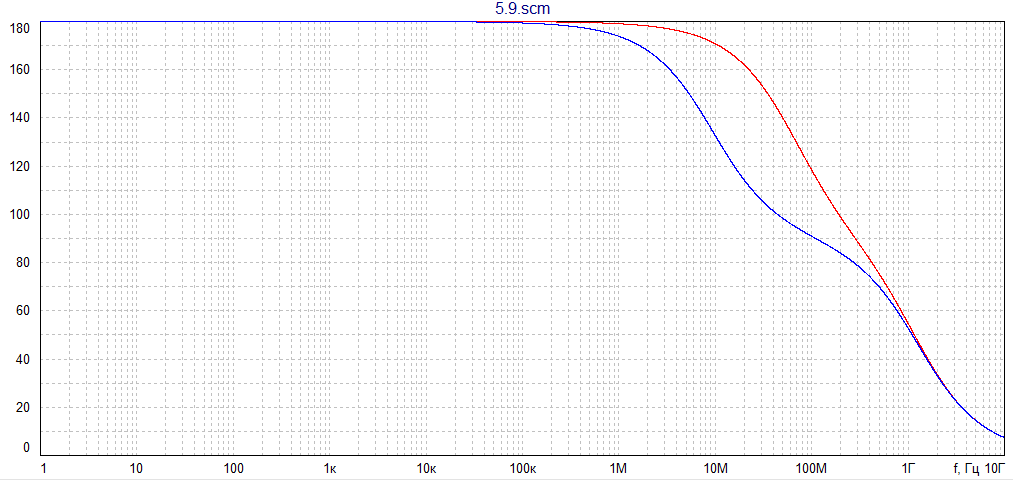
\includegraphics[scale=0.6]{8.png}
        \end{center}
        \caption{График ФЧХ. Красная линия - $K_F$=10, Синяя линия- $K_F$=100.}
    \end{figure}

    \textbf{Вывод по заданию:}

    \begin{itemize}
        \item Значения коэффициента усиления, полученные по АЧХ и теоретически рассчитанные, практически совпадают.
    При этом отношение рассчитанных $K_{f1}$ и $K_{f2}$ и полученных из АЧХ совпадают.
        \item При увеличении $К_F$ наблюдается уменьшение рабочего диапазона частот.
    \end{itemize}

    \begin{center}
        \textbf{Задание 4.}
    \end{center}

    Инвертирующий усилитель с высоким входным сопротивлением
    
    Для получения высокого входного сопротивления в инвертирующем 
    усилителе используется Т-образная цепь ОС. Резисторы, подключаемые ко
    входу ОУ, выбираются высокоомными (например 1 МОм). Два других
    используются для управления коэффициентом усиления.

    Коэффициент усиления такой схемы рассчитываются следующим образом:

    \begin{center}
        $K_F=\frac{\mu(R_4(R_5+R_6)+R_5R_6))}{\mu R_3R_6+(R_3+R_4)(R_5+R_6)+R_5R_6)}\approx \frac{(1+\frac{R_5}{R_6})R_4}{R_3}$
    \end{center}
    \begin{figure}[h!]
        \begin{center}
            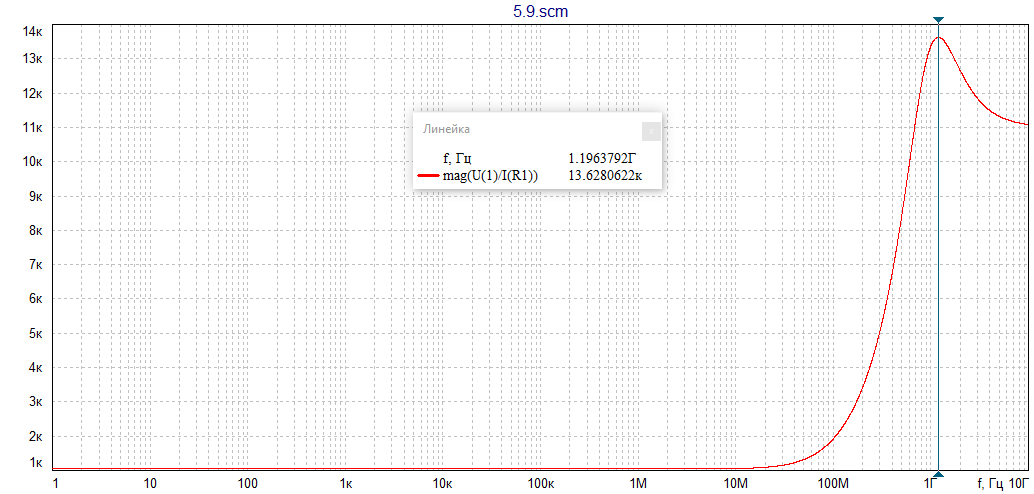
\includegraphics[width=15cm,height=5cm]{10.png}
        \end{center}
        \caption{График входного сопротивления инвертирующего усилителя.}
    \end{figure}

    Входное сопротивление инвертирующего усилителя равно 13,6кОм

    \textbf{Вывод по заданию:}

    \begin{itemize}
        \item Входное сопротивление инвертирующего усилителя, вычисленное в Fastmean, практическии совпадает с теоретическим.
    \end{itemize}

    \newpage
    \begin{center}
        \textbf{Задание 5.}
    \end{center}
    \begin{figure}[h!]
        \begin{center}
            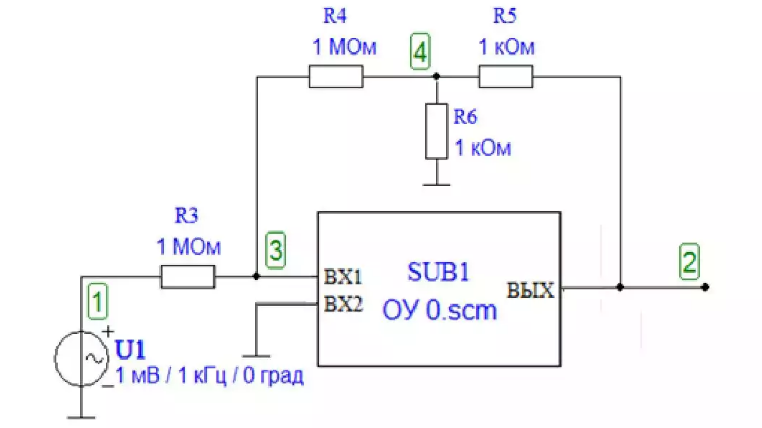
\includegraphics[scale=0.4]{11.png}
        \end{center}
        \caption{Инвертирующий ОУ с высоким входным сопротивлением.}
        \begin{center}
            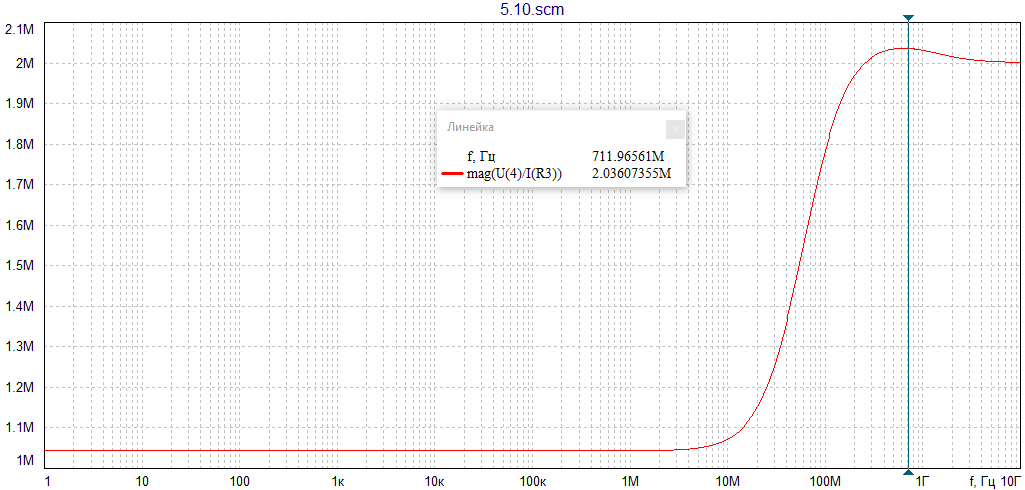
\includegraphics[scale=0.5]{12.png}
        \end{center}
        \caption{График входного сопротивления.}
        \vspace{-0.7cm}
    \end{figure}

    Входное сопротивление инвертирующего ОУ с высоким входным сопротивлением равно 2.04 МОм.

    Рассчитать элементы цепи ОС по заданному коэффициенту усиления $K_F$ = 100
    и $K_F$ = 10.
    \begin{multicols}{2}
        \begin{tabbing}
            \noindent $K_F$ = 10\=\\
            \>$K_F$ = (1+R5/R6)*R4/R3\\
            \>R3 = 1000 Ом\\
            \>R3 = R4 = 1 МОм\\
            \>R5 = 9*R6 = 9 кОм\\\\

            $K_F$ = 100\=\\
            \>$K_F$ = (1+R5/R6)*R4/R3\\
            \>R3 = 1000 Ом\\
            \>R3 = R4 = 1 МОм\\
            \>R5 = 99*R6 = 99 кОм\\
        \end{tabbing}
    \end{multicols}
    \begin{figure}[h!]
        \begin{center}
            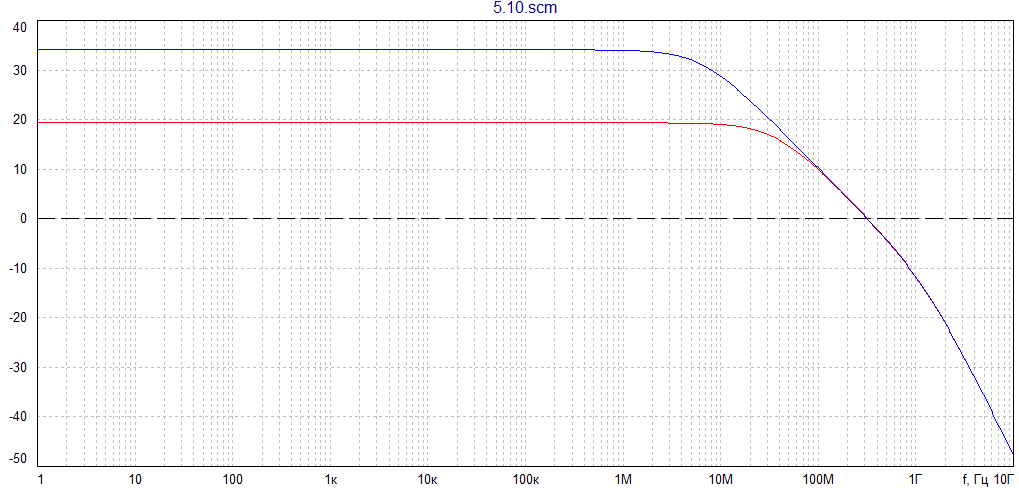
\includegraphics[scale=0.5]{13.png}
        \end{center}
        \vspace{-0.7cm}
        \caption{График АЧХ. Красная линия - $K_F$=10, Синяя линия - $K_F$=100.}
    \end{figure}
   
    \emph{Неинвертирующий усилитель на ОУ} получается при подаче сигнала 
    на его прямой вход. На практике вызывает интерес частный случай 
    такого включения — операционный повторитель (ОП) (рис. 16).

    \begin{figure}[h!]
        \begin{center}
            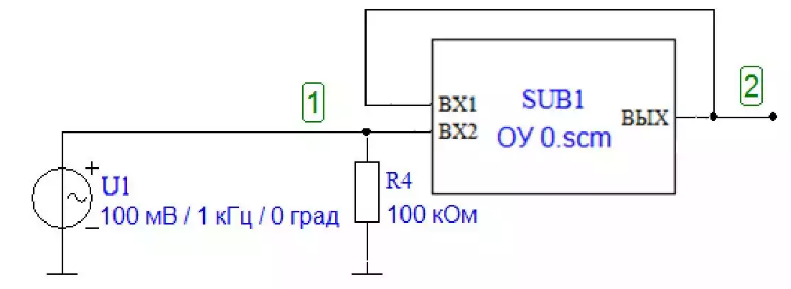
\includegraphics[scale=0.5]{14.png}
        \end{center}
        \vspace{-0.7cm}
        \caption{График АЧХ. Красная линия - $К_F$=10, Синяя линия - $К_F$=100.}
    \end{figure}

    Режим ОП получается в неинвертирующем усилителе при R2 = 0. Выход ОУ 
    непосредственно соединяется с инверсным входом, использование резистора 
    R1 в этом случае теряет смысл. Резистор R4 необходим для протекания 
    входного постоянного тока ОУ. Его сопротивление может составлять 
    десятки и сотни кОм. Оно определяет входное сопротивление ОП. При этом 
    следует помнить о входных токах ОУ.

    \textbf{Вывод по заданию:}

    \begin{itemize}
        \item Входное сопротивление инвертирующего усилителя с высоким входным сопротивлением почти на 3 порядка больше, чем у инвертирующего усилителя.
    \end{itemize}

    \newpage

    \begin{center}
        \textbf{Задание 6.}
    \end{center}
    \vspace{-0,5cm}
    \begin{figure}[h!]
        \begin{center}
            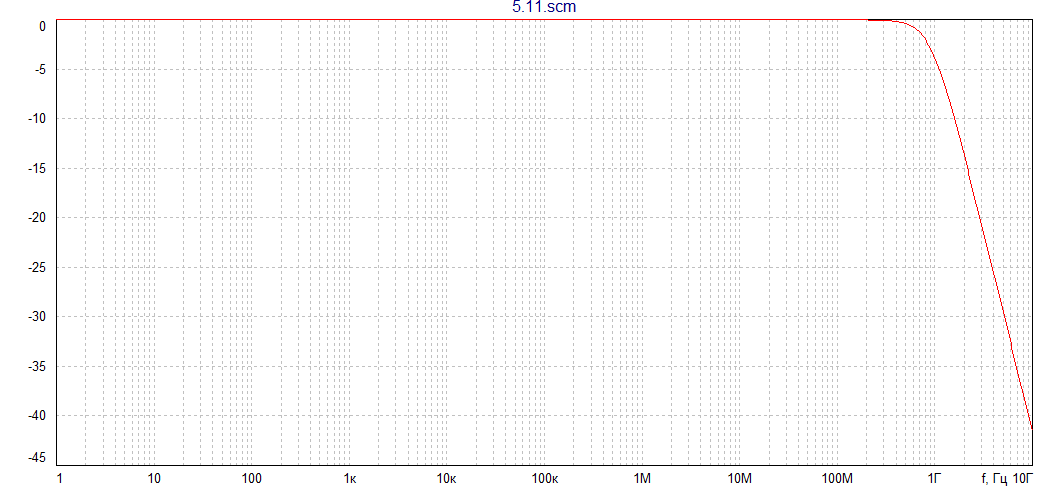
\includegraphics[scale=0.5]{15.png}
        \end{center}
        \vspace{-0.7cm}
        \caption{График АЧХ ОП.}
    \end{figure}

    \vspace{-0,5cm}
    \textbf{Вывод по заданию:}
    \vspace{-0,5cm}

    \begin{itemize}
        \item В отличие от АЧХ усиления без ОС, АЧХ операционного повторителя имеет большую рабочую полосу частот, а максимум его АЧХ равен 0 дБ.
    \end{itemize}

    \vspace{-0,5cm}
    \begin{center}
        \textbf{3.2.1.2. Характеристики во временной области.}
    \end{center}
    \vspace{-0,5cm}

    Переходную характеристику (ПХ) усилителя получаем при подаче на его 
    вход напряжения прямоугольной формы. Для этого в схемах на рис. 5 и 16 
    необходимо переключить источник сигналов с гармонических колебаний на 
    меандр. Задать двухполярный сигнал ±1 мВ и длительность импульса $t_\text{и}$= 
    25 мкс.

    \vspace{-0,5cm}
    \begin{center}
        \textbf{Задание 7.}
    \end{center}
    
    \begin{figure}[h!]
        \begin{center}
            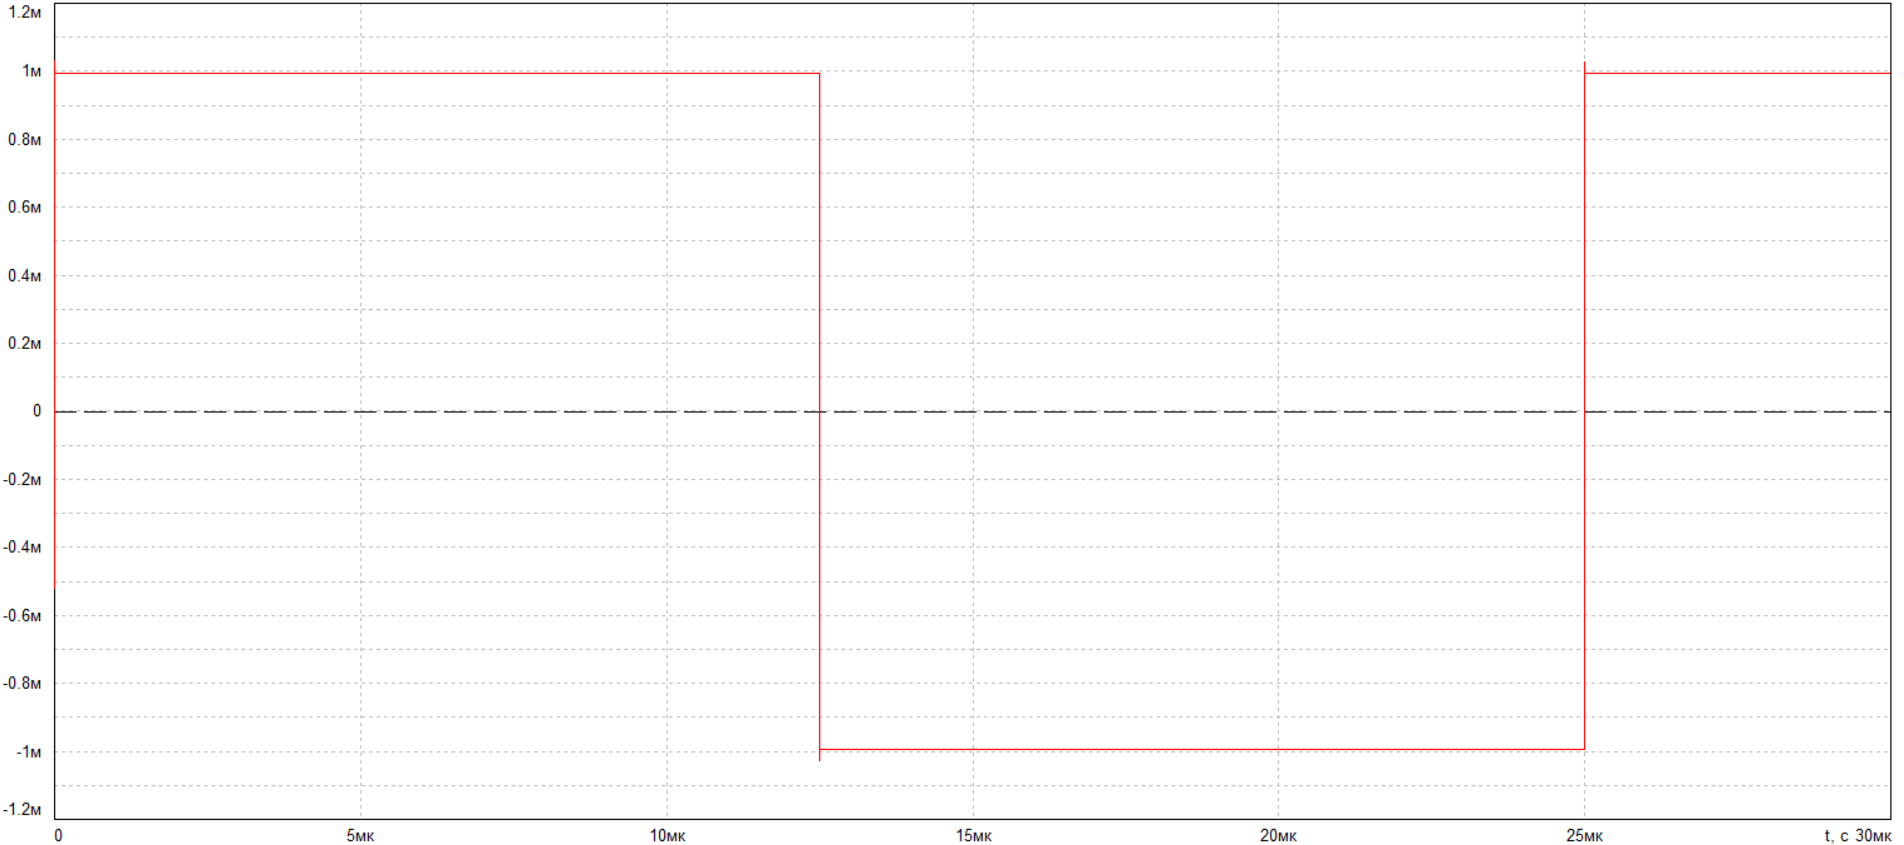
\includegraphics[scale=0.24]{16.png}
        \end{center}
        \vspace{-0.7cm}
        \caption{График ПХ операционного повторителя.}
    \end{figure}
    \vspace{2cm}

    \begin{figure}[h!]
        \begin{center}
            
\includegraphics[scale=0.25]{17.png}
        \end{center}
        \vspace{-0.7cm}
        \caption{График ПХ инвертирующего ОУ с высоким входным сопротивлением.}
    \end{figure}

    \textbf{Вывод по заданию:}

    \begin{itemize}
        \item По ПХ операционного повторителя видно, что она практически в точности повторяет входной сигнал источника напряжения.
        \item По ПХ инвертирующего усилителя можно сделать вывод о том, что данное устроиство инфертирует входной сгнал и усиливает его в $K_f$ раз.
    \end{itemize}


    \begin{center}
        \textbf{3.2.2. Схемы на ОУ с частотно-зависимой ОС.}
    \end{center}

    Из огромного разнообразия схем ОУ с частотно-зависимыми цепями ОС для 
    лабораторного исследования выбраны только две.

    Одна из них представляет собой интегратор (рис. 20, а), 
    другая — дифференциатор (рис. 20, 6). Соответствующие функции 
    определяются RC-элементами. Резисторы $R_0$ выполняют вспомогательные 
    функции. В интеграторе $R_0$ обеспечивает необходимую ОС на постоянном 
    токе, в дифференциаторе — необходимый запас по фазе.

    \begin{figure}[h!]
        \begin{center}
            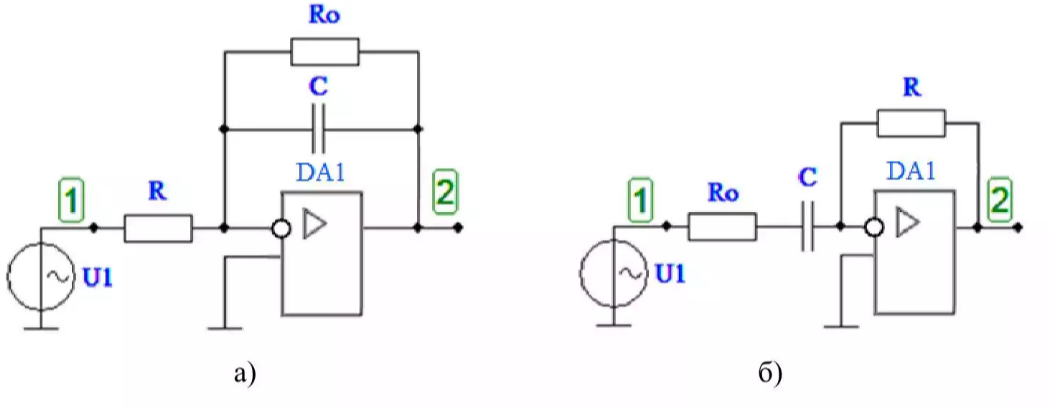
\includegraphics[scale=0.4]{18.png}
        \end{center}
        \vspace{-0.7cm}
        \caption{ОУ в режиме интегрирования (а) и дифференцирования (б).}
    \end{figure}

    \newpage
    \begin{center}
        \textbf{3.2.2.1. Характеристики в частотной области.}
    \end{center}

    \begin{figure}[h!]
        \begin{center}
            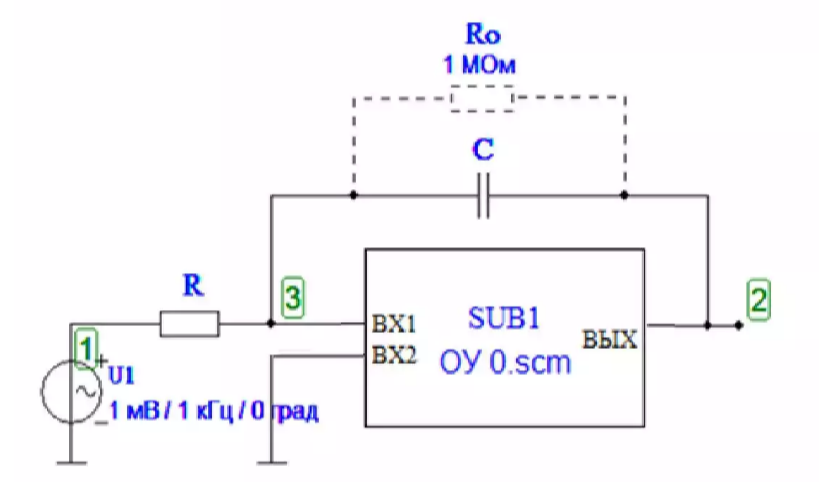
\includegraphics[scale=0.5]{19.png}
        \end{center}
        \vspace{-0.7cm}
        \caption{Схема интегратора.}
    \end{figure}

    \newpage
    \begin{center}
        \textbf{Задание 8.}
    \end{center}

    \begin{figure}[h!]
        \begin{center}
            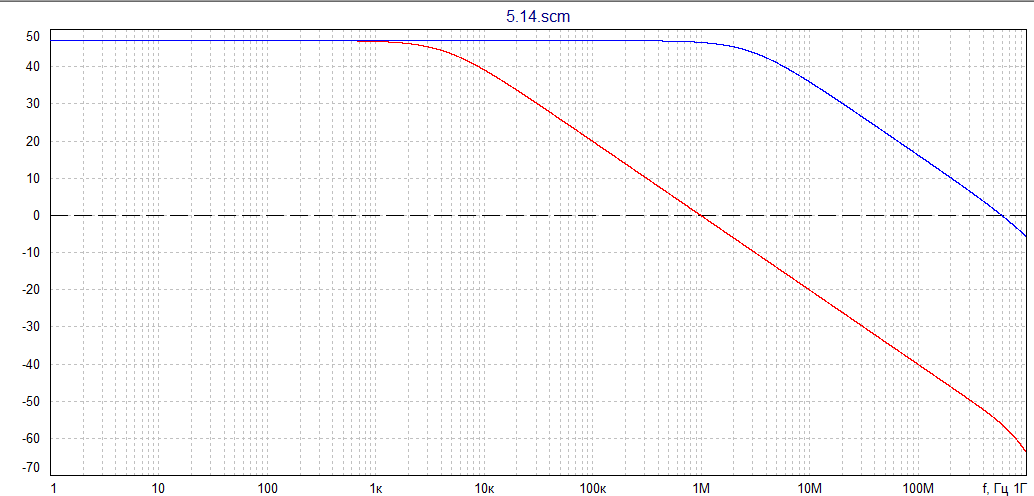
\includegraphics[scale=0.6]{20.png}
        \end{center}
        \vspace{-0.7cm}
        \caption{График АЧХ интегратора (красная линия) и АЧХ ОУ без ОС (синяя линия).}
    \end{figure}

    \begin{figure}[h!]
        \begin{center}
            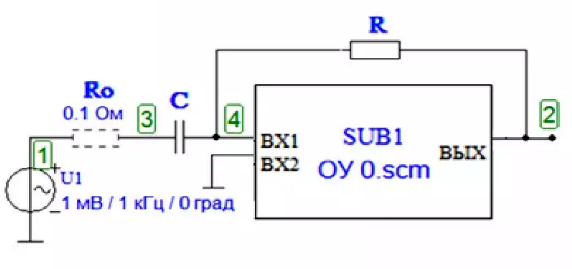
\includegraphics[scale=0.6]{21.png}
        \end{center}
        \vspace{-0.7cm}
        \caption{ Схема дифференциатора.}
    \end{figure}

    \textbf{Вывод по заданию:}

    \begin{itemize}
        \item По АЧХ схемы видно, что выполняется условие падения АЧХ на 6дБ/октава, а значит, что схема действительно работает как интегратор.
    \end{itemize}

    \newpage
    \begin{center}
        \textbf{Задание 9.}
    \end{center}

    \begin{figure}[h!]
        \captionsetup{justification=centering}
        \begin{center}
            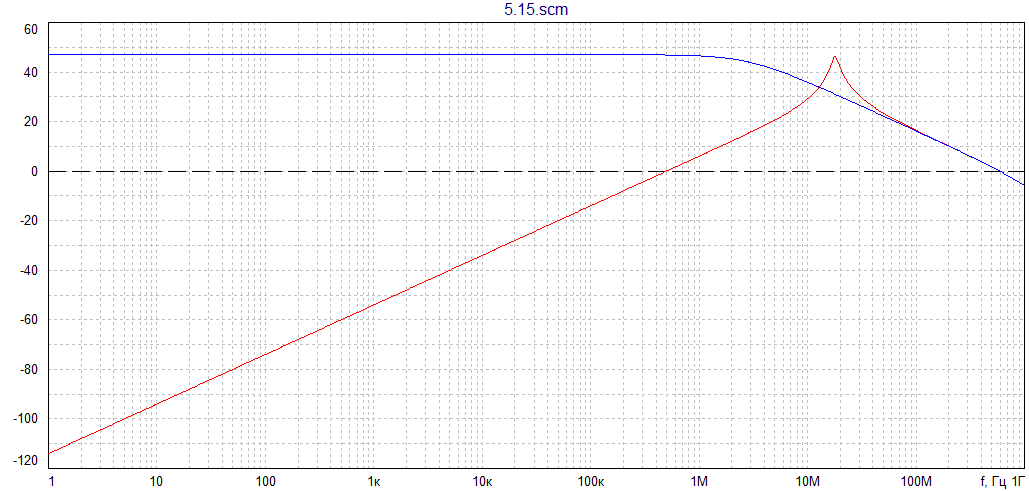
\includegraphics[scale=0.6]{22.png}
        \end{center}
        \vspace{-0.7cm}
        \caption{График АЧХ дифференциатора (красная линия) и АЧХ ОУ без ОС (синяя линия).} 
    \end{figure}
    \begin{figure}[h!]
        \captionsetup{justification=centering}
        \begin{center}
            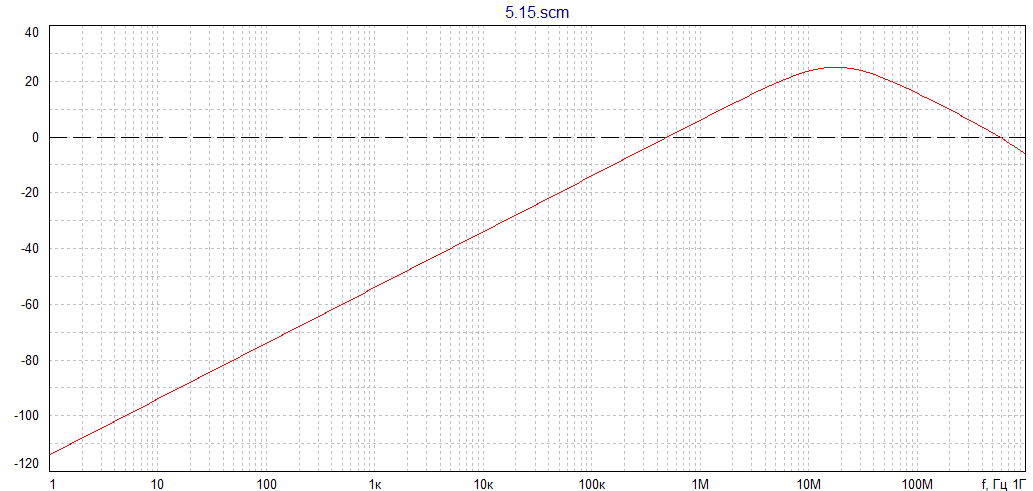
\includegraphics[scale=0.6]{23.png}
        \end{center}
        \vspace{-0.7cm}
        \caption{График АЧХ дифференциатора при $R_0$ = 240 Ом – сопротивлении, при котором подъем на АЧХ перестает иметь место.} 
    \end{figure}
 
    В реальной схеме с ОУ выполнить измерения с разомкнутой петлей ОС 
    весьма сложно из-за чрезвычайно высокого коэффициента усиления ОУ и 
    необходимости сохранения нулевых потенциалов на постоянном напряжении. 
    Использование ПК существенно облегчает решение этой задачи. На рис. 26 
    показан вариант выполнения разрыва петли ОС на ПК в схеме на рис. 23.

    \begin{figure}
        \begin{center}
            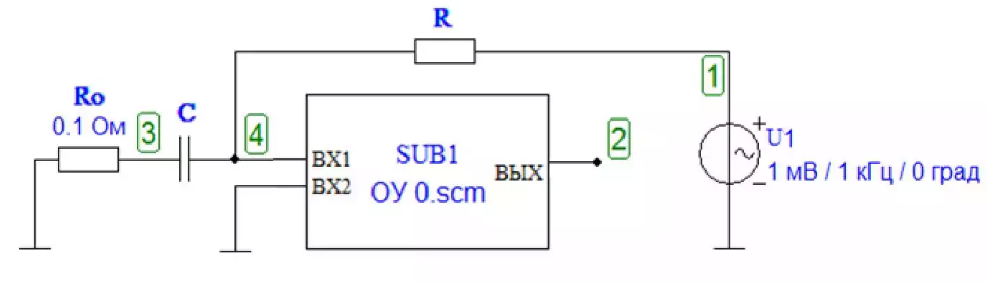
\includegraphics[scale=0.5]{24.png}
        \end{center}
        \vspace{-0.7cm}
        \caption{Схема дифференциатора с разомкнутой петлей ОС.}
    \end{figure}
    
    \begin{figure}
        \textbf{Вывод по заданию:}

        \begin{itemize}
            \item Изменение значения $R_0$ сглаживает выброс на АЧХ, а при значении $R_0$ = 240 Ом данный выброс перестает иметь место. Помимо этого, данное сопротивление не оказывает никаого влияния на рабочий диапазон частот.
        \end{itemize}
    \end{figure}
  
    \newpage
    \begin{center}
        \textbf{Задание 10.}
    \end{center}
    \vspace{-0.5cm}
    \begin{figure}[h!]
        \captionsetup{justification=centering}
        \begin{center}
            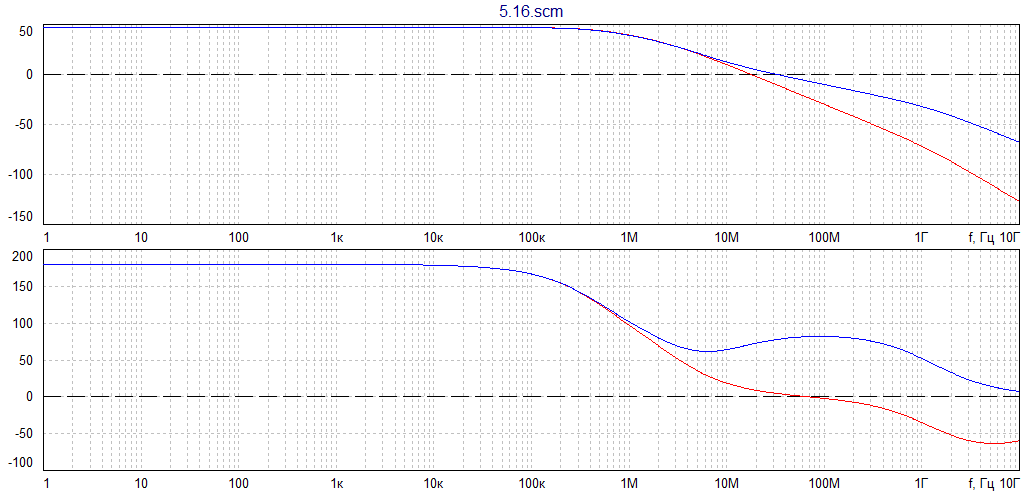
\includegraphics[scale=0.5]{25.png}
        \end{center}
        \vspace{-0.7cm}
        \caption{График АЧХ петлевого усиления дифференциатора Красная линия – $R_0$=0.1Ом, синяя линия - $R_0$=240Ом.}
    \end{figure}
 
    \begin{figure}[h!]
        \begin{center}
           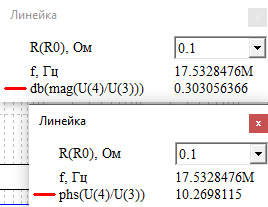
\includegraphics[scale=0.8]{26.png}
           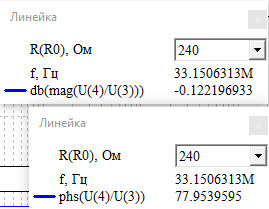
\includegraphics[scale=0.8]{27.png}           
        \end{center}
        \vspace{-0.7cm}
        \caption{Значения АЧХ и ФЧХ, при значении АЧХ = 0Дб}
        \vspace{-0.5cm}
    \end{figure}   

    \vspace{1.5cm}
    \textbf{Вывод по заданию:}

    \begin{itemize}
        \item  Изменение $R_0$ практически не влияет на значение частоты единичного усиления, а на ФЧХ происходит значительное изменение запаса устойчивости по
фазе. При этом, чем больше данный запас, тем устойчивее усилитель.
    \end{itemize}
 
    \begin{center}
        \textbf{3.2.2.2. Характеристики во временной области.}
    \end{center}

    Переходную характеристику (ПХ) получаем при подаче на вход исследуемой 
    схемы напряжения прямоугольной формы. Для этого в схемах на рис. 21 и 
    23 необходимо переключить источник сигналов с гармонических колебаний 
    на меандр. Задать двухполярный сигнал ±1 мВ. Частота следования 
    прямоугольных импульсов устанавливается в зависимости от их 
    длительности импульса $t_\text{и}$ = $\frac{1}{2f}$ для интегратора и для 
    дифференциатора $t_\text{и}$ = 500 мкс.

    \begin{center}
        \textbf{Задание 11.}
    \end{center}
    
    \begin{figure}[h!]
        \begin{center}
            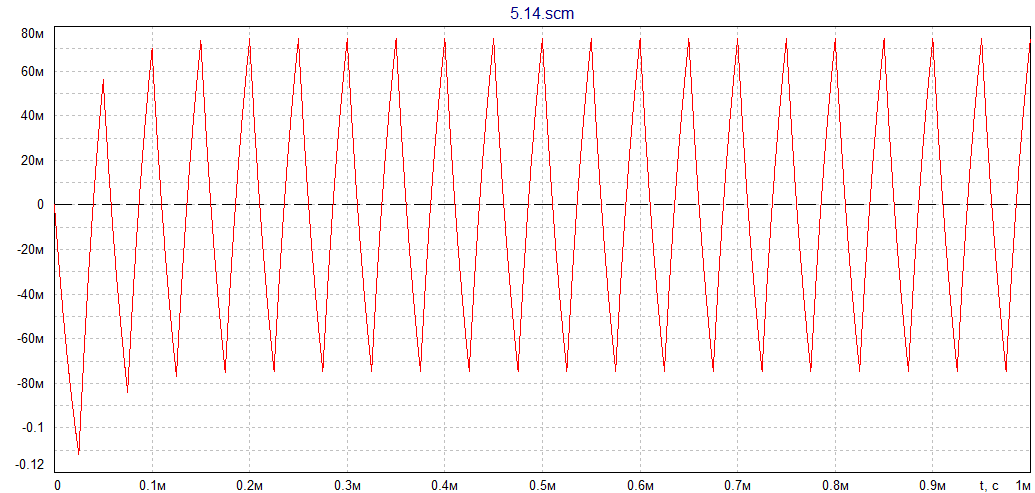
\includegraphics[scale=0.5]{28.png}
        \end{center}
        \vspace{-0.7cm}
        \caption{График линейного закона интегрирования.}
    \end{figure}

    \begin{figure}[h!]
        \begin{center}
            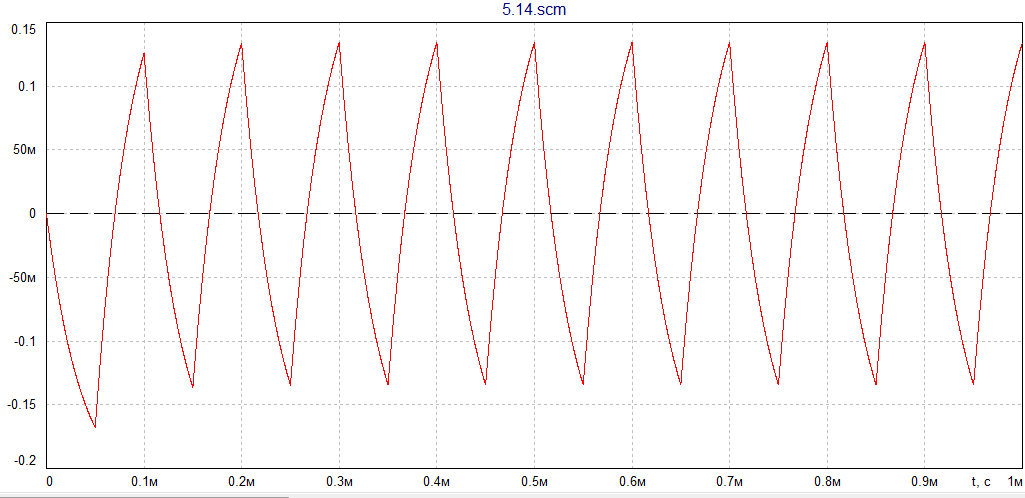
\includegraphics[scale=0.5]{29.png}
        \end{center}
        \vspace{-0.7cm}
        \caption{График экспоненциального закона интегрирования.}
        $t_\text{имакс}$=500 мкс
    \end{figure}
    \begin{figure}[h!]
       \textbf{Вывод по заданию:}

        \begin{itemize}
            \item При увеличении длительности импульса, линейный закон 
            интегрирования переходит в экспоненциальный.
            \item При подаче на вход интегратора прямоугольных импульсов на 
            выходе наблюдается пилообразный сигнал
        \end{itemize}
    \end{figure}

    \newpage
    \begin{center}
        \textbf{Задание 12.}
    \end{center}

    \begin{figure}[h!]
        \begin{center}
            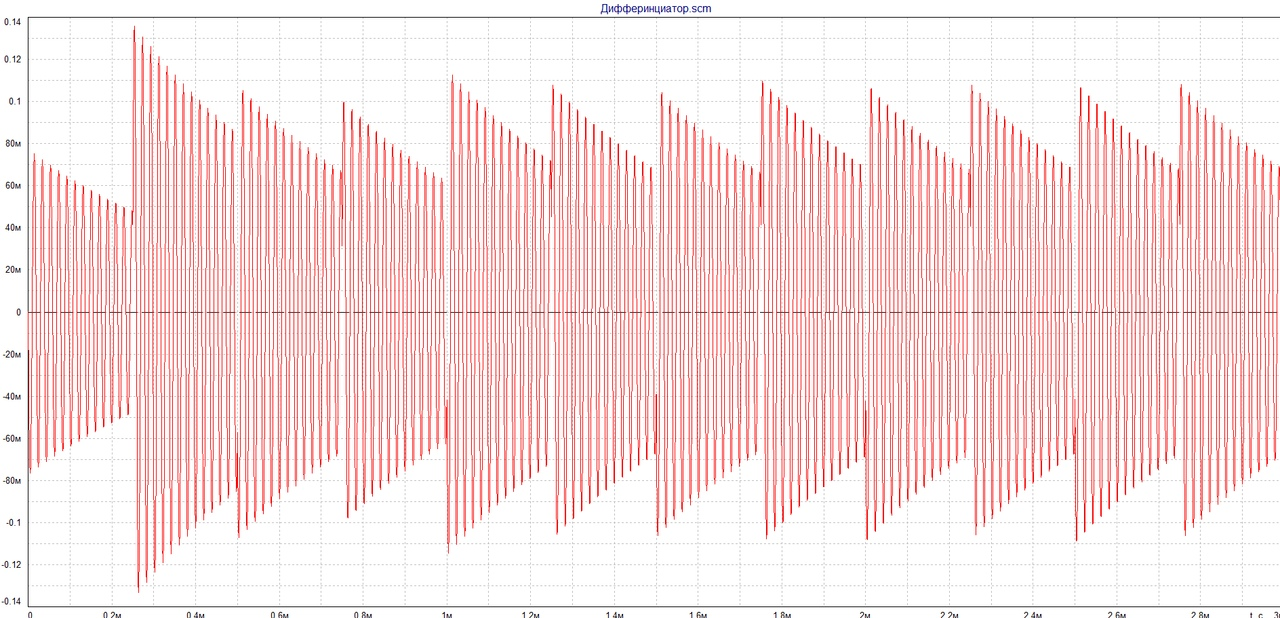
\includegraphics[scale=0.3]{30.jpeg}
        \end{center}
        \vspace{-0.7cm}
        \caption{График ПХ при $R_0$ = 0.1 Ом, запас устойчивости по фазе равен 10 градусов.}
    \end{figure}

    \begin{center}
        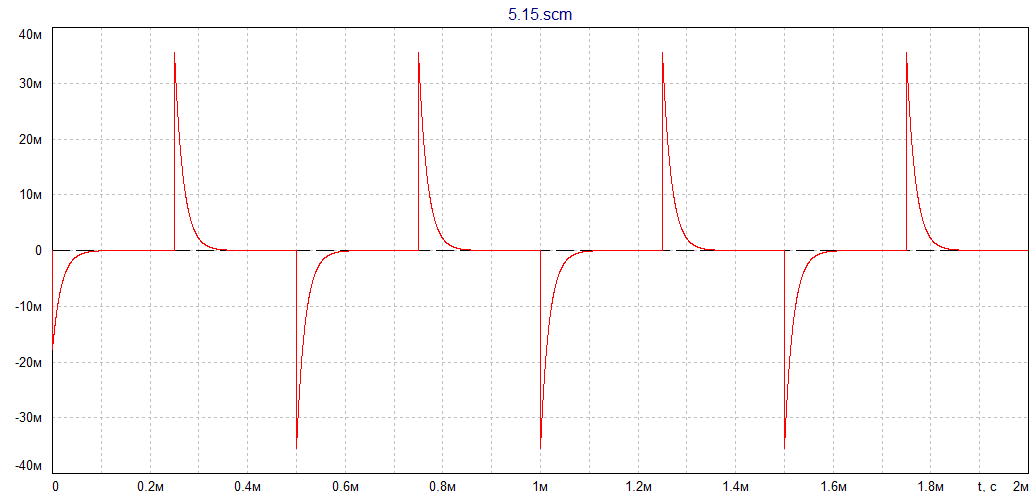
\includegraphics[scale=0.5]{31.png}
    \end{center}
    \vspace{-0.7cm}
    Рис.28: График ПХ при $R_0$ = 240 Ом, запас устойчивости по фазе 78 градусов.

   \textbf{Вывод по заданию:}
   \begin{itemize}
       \item По полученным ПХ, можно сделать вывод о том, что перед нами дифференциатор. Изменение запаса по фазе влияет на его ПХ, а именно при $R_0$=0.1 Ом (усилитель практически самовозбужден) наблюдается потеря устойчивости и искажение выходного сигнала, а при $R_0$=240 Ом его выходная характеристика практически точно отображает дифференцированное значение сигнала.
   \end{itemize}

    \textbf{Вывод:} во время выполнения лабораторной работы были изучены 
    схемотехнические особенности построения интегральных ОУ, принцип 
    построения макромодели в частотной области и исследованы влияние 
    внешних цепей ОС на характеристики устройств с ОУ. 
    

\end{document}